\subsection{Analisis Kebutuhan Sistem}
\label{sec:analisis-kebutuhan-sistem}

Berdasarkan bagian \ref{sec:analisis-solusi}, Kubernetes menjadi pilihan solusi yang digunakan karena memiliki berbagai kelebihan dibandingkan dengan pendekatan lain terutama dalam hal \textit{targeted deployment}. Kubernetes, sebagai sistem orkestrasi kontainer yang matang dan luas digunakan, menawarkan fitur dan kemampuan yang cocok untuk mengatasi tantangan yang dihadapi dalam lingkungan IoT yang heterogen dan terdistribusi terutama dalam masalah skalabilitas, \textit{ready to use}, serta memakan waktu yang minimal sehingga solusi ini merupakan solusi paling \textit{feasible} yang dapat diimplementasikan.

PERISAI akan menggunakan kubernetes sebagai sistem orkestrasi dalam mengatur banyak perangkat. Namun, sebelum membuat arsitektur PERISAI, perlu dilakukan analisis kebutuhan untuk sistem yang diperlukan. PERISAI akan digunakan pada skala besar sehingga perlu adanya sebuah organisasi yang bertanggung jawab atas seluruh perangkat yang dimiliki. Selain itu, untuk melakukan manajemen perangkat pasti dibutuhkan satu atau lebih \textit{user} yang dapat melakukan proses manajemen perangkat ataupun \textit{remote deployment}. PERISAI juga harrus dapat mengelompkan satu atau lebih perangkat untuk memudahkan proses \textit{deployment}. Proses \textit{deployment} dapat dilakukan untuk satu perangkat atau lebih serta melakukan \textit{deployment} kepada beberapa grup yang telah dikelompokan. Berangkat dari permasalahan tersebut, akan diuraikan kebutuhan sistem yang terbagi menjadi kebutuhan fungsional dan non-fungsional.

\subsubsection{Deskripsi sistem}
Sistem yang dibuat merupakan sebuah sistem yang dapat melakukan \textit{remote deployment} ke perangkat yang terhubung ataupun ke sebagian perangkat yang diinginkan. Sistem memiliki dua komponen utama yaitu \textit{dashboard} sebagai \textit{frontend} serta API sebagai \textit{backend}. Komponen \textit{backend} ini memiliki dua modul eksternal dan satu modul internal. Kubernetes dan \textit{database} sebagai modul eksternal serta server sebagai penghubung modul eksternal dengan modul internal. Modul Kubernetes terhubung ke kluster yang diinginkan untuk melakukan proses \textit{remote deployment} ke masing-masing perangkat yang terhubung. Ilustrasi secara kasar dapat dilihat pada gambar \ref{fig:gambaran-umum-arsitektur}.

\begin{figure}[ht]
  \centering
  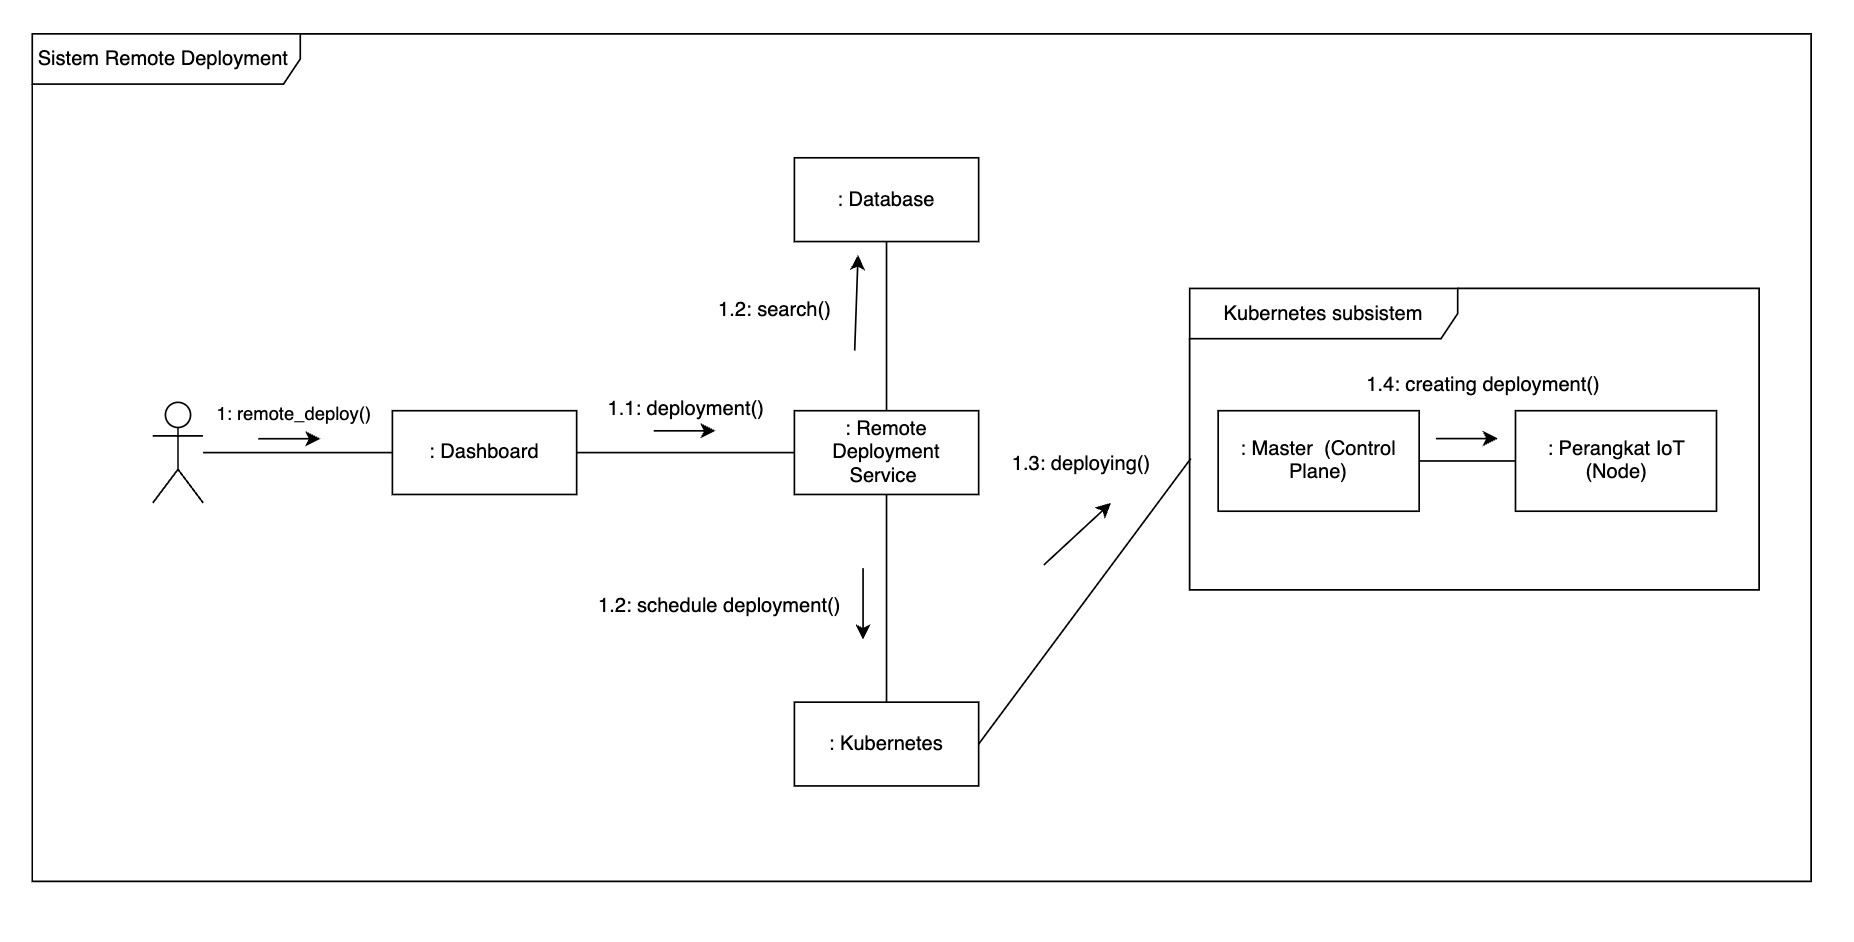
\includegraphics[width=1\textwidth]{resources/chapter-3/gambaran-umum-arsitektur-updated.jpg}
  \caption{Gambaran Umum Arsitektur PERISAI}
  \label{fig:gambaran-umum-arsitektur}
\end{figure}

\pagebreak
\subsubsection{Karakteristik Pengguna}
Berdasarkan hasil analisis, terdapat dua pengguna pada sistem ini, yaitu pengguna dan administrator. Penjelasan lebih detail dapat dilihat pada tabel \ref{tab:karakteristik-pengguna}.

\bgroup
\begin{table}[ht]
  \def\arraystretch{1.7}
  \caption{Karakteristik Pengguna}
  \label{tab:karakteristik-pengguna}
  \centering
  \begin{tabular}{|p{2cm}|p{8cm}|}
    \hline
    Kategori Pengguna & Hak akses                                                                                                                                                                                                                                                                           \\
    \hline
    \textit{User}     & \textit{User} dapat melakukan login, registrasi, melihat \textit{user} lain di satu perusahaan, melakukan manajemen perangkat, melakukan manajemen groups, melakukan manajemen \textit{deployment}, melakukan \textit{remote deployment}, serta melihat riwayat \textit{deployment} \\
    \hline
    Admin             & Admin dapat melakukan manajemen perusahaan, manajemen user, serta seluruh kegiatan yang user dapat lakukan                                                                                                                                                                          \\
    \hline
  \end{tabular}
\end{table}
\egroup

\subsubsection{Kebutuhan Fungsional}
Sistem memiliki beberapa kebutuhan fungsional yang dipetakan dalam bentuk tabel yang dapat dilihat pada lampiran \ref{tab:kebutuhan-fungsional}. Semua kebutuhan fungsional memiliki ID yang diawali dengan huruf F lalu diikuti dengan dua angka.



\subsubsection{Kebutuhan Non-Fungsional}
Sistem memiliki 2 parameter kebutuhan non-fungsional yang dapat dilihat pada tabel \ref{tab:kebutuhan-non-fungsional}. Semua kebutuhan non-fungsional memiliki awalan ID NF lalu diikuti oleh dua angka.

\bgroup
\begin{table}[ht]
  \def\arraystretch{1.7}
  \caption{Kebutuhan Non-Fungsional}
  \label{tab:kebutuhan-non-fungsional}
  \centering
  \begin{tabular}{|c|p{3cm}|p{8cm}|}
    \hline
    ID   & Parameter            & Kebutuhan                                                                                                                                                                                                                          \\
    \hline
    NF01 & \textit{Security}    & Sistem menjamin keamanan dari \textit{service} dengan cara menyediakan validasi pada \textit{middleware} serta setiap \textit{request} dapat terhindar dari serangan. Hanya \textit{user} yang terautentikasi yang bisa mengakses. \\
    \hline
    NF02 & \textit{Portability} & Sistem dapat diakses dimana saja melalui perangkat laptop.                                                                                                                                                                         \\
    \hline
  \end{tabular}
\end{table}
\egroup

\subsubsection{Model \textit{Use case}}
\label{subsec:model-usecase}
Dari beberapa kebutuhan fungsional serta karakteristik pengguna, dapat dibuat \textit{use case} yang mengelompokkan serta menggambarkan relasi antara aktor dan aksi yang dapat dilakukan. \textit{Use case} memiliki identifikasi yang berawalan dengan UC diikuti oleh dua angka. \textit{Use case} dapat dilihat secara detail pada lampiran \ref{tab:penjelasan-usecase-diagram}.

Dari pemetaan \textit{use case} pada lampiran \ref{tab:penjelasan-usecase-diagram}, dapat dibuat sebuah diagram yang menghubungkan relasi antara aktor dengan \textit{use case}-nya. Relasi  aktor dengan kapabilitas fungsional sistem dapat dilihat pada diagram use case di Gambar \ref{fig:usecase-diagram}.

\begin{figure}[ht]
  \centering
  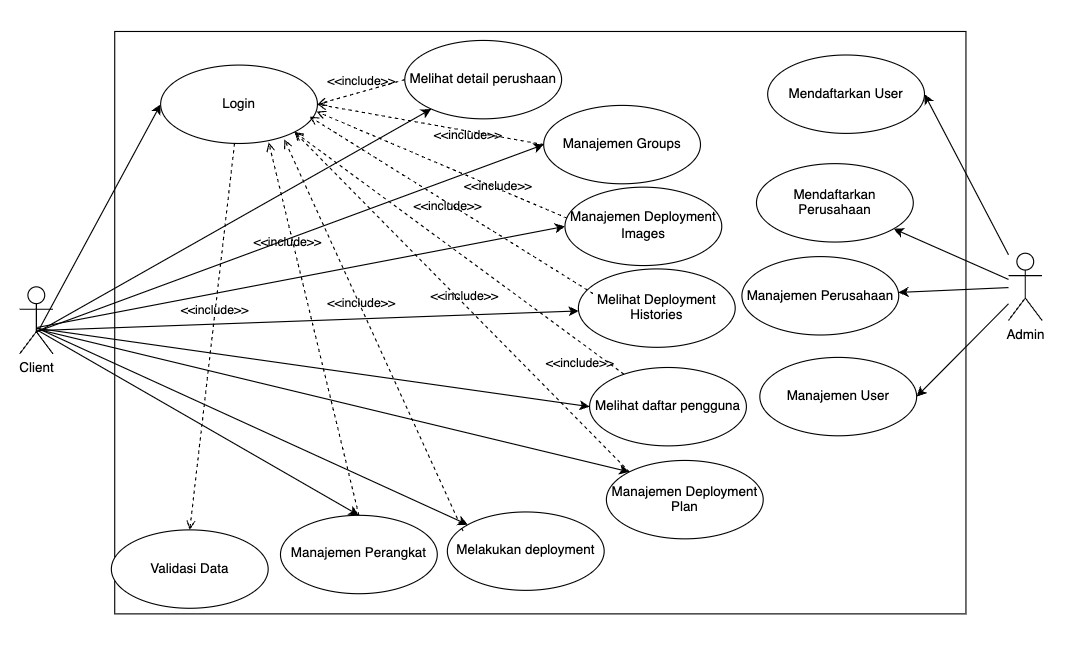
\includegraphics[width=1\textwidth]{resources/chapter-3/usecase-diagram.jpg}
  \caption{Usecase Diagram}
  \label{fig:usecase-diagram}
\end{figure}

\pagebreak
